\documentclass{a4beamer}
%% Lectures - common definitions

\usextensions{tikz}
\usetikzlibrary{shapes.multipart,shapes.callouts,shapes.geometric}
\input{fix-callouts.inc} % Fixes absolute positioning of rectangle callouts

\newif\ifbigpages \bigpagesfalse
\ifdim\paperwidth >20cm
	\bigpagestrue
\fi

\tikzset{%
	note/.style={rectangle callout,draw=none,callout pointer width=1em,%
		align=flush left,font=\footnotesize,inner sep=0.5em,%
		fill=blue!15,fill opacity=0.95,text opacity=1.0,callout absolute pointer=#1},
	node distance=2em and 2.75em
}
\ifbigpages
	% Scale all arrow tips by the factor of 2.5
	\let\old@pgf@arrow@call=\pgf@arrow@call
	\def\pgf@arrow@call#1{%
		\@tempdima=\pgflinewidth%
		\pgfsetlinewidth{2.5\pgflinewidth}%
		\old@pgf@arrow@call{#1}%
		\pgfsetlinewidth{\@tempdima}%
	}
	\def\pgfarrowsleftextend#1{\pgfmathsetlength{\pgf@xa}{1.5*#1}}
	\def\pgfarrowsrightextend#1{\pgfmathsetlength{\pgf@xb}{1.5*#1}}
\fi

%% Load listings package
\usepackage{listings}

%% Are we inside a comment?
\newif\iflstcomment \lstcommentfalse

\lstset{%
	tabsize=4,
	showstringspaces=false,
	basicstyle=\linespread{1.25}\ttfamily\small,
	keywordstyle=\bfseries,
	commentstyle=\lstcommentstyle,
	numbers=left,
	numberstyle=\footnotesize\color{gray},
	xleftmargin=2.5em,
	extendedchars=true,
	escapechar=\$,
	escapebegin=\iflstcomment\begingroup\lstcommentstyle\fi,
	escapeend=\iflstcomment\endgroup\fi
}

\def\lstcommentstyle{\color{gray}}

\lst@AddToHook{AfterBeginComment}{\global\lstcommenttrue}
\let\orig@lst@EndComment=\lst@EndComment
\def\lst@EndComment{\global\lstcommentfalse\orig@lst@EndComment}
\lst@AddToHookAtTop{EOL}{%
	\lst@ifLmode\global\lstcommentfalse\fi% XXX Sloppy way to determine comment end
}

%% Python with docstrings treated as comments
\lstdefinelanguage[doc]{python}[]{python}{%
	deletestring=[s]{"""}{"""},%
	morecomment=[s]{"""}{"""}%
}%

%% JavaScript language
\lstdefinelanguage{javascript}%
	{morekeywords={break,case,catch,%
		const,constructor,continue,default,do,else,false,%
		finally,for,function,if,in,instanceof,%
		new,null,prototype,%
		return,switch,this,throw,%
		true,try,typeof,var,while},%
	sensitive,%
	morecomment=[l]//,%
	morecomment=[s]{/*}{*/},%
	morestring=[b]",%
	morestring=[b]',%
}[keywords,comments,strings]%

%% C# language (4.0?)
\lstdefinelanguage{csharp}%
	{morekeywords={abstract,as,%
		base,bool,byte,case,catch,char,%
		checked,class,const,continue,%
		decimal,default,delegate,do,double,%
		else,enum,event,explicit,extern,%
		false,finally,fixed,float,for,foreach,%
		goto,if,implicit,in,int,interface,%
		internal,is,lock,long,%
		namespace,new,null,object,operator,out,%
		override,params,private,protected,public,%
		readonly,ref,return,sbyte,sealed,%
		short,sizeof,stackalloc,static,string,%
		struct,switch,this,throw,true,try,%
		typeof,uint,ulong,unchecked,unsafe,ushort,%
		using,virtual,void,volatile,while%
	},%
	sensitive,%
	morecomment=[l]//,%
	morecomment=[s]{/*}{*/},%
	morestring=[b]",%
	morestring=[b]',%
}[keywords,comments,strings]%

%% Translation for fact environment
\deftranslation[to=russian]{Fact}{Наблюдение}

%% Inline code snippets
\def\code#1{\texttt{#1}}
\def\codekw#1{\code{\textbf{#1}}}

\def\quoteauthor#1{\par\footnotesize\upshape\hfill—~#1}

%% English term
\def\engterm#1{(англ. \textit{#1})}
%% Term with explanation below (to be used in diagrams)
\def\termwithexpl#1#2{#1\strut{}\\\small\color{gray}(\textit{#2})\strut{}}
%% External link
\def\extlink#1#2{\href{#1}{\color[rgb]{0.7,0.7,1.0}\dashbar{#2}}}
%% Internal link
\def\inlink#1#2{\hyperlink{#1}{\color[rgb]{0.7,0.7,1.0}\dashbar{#2}}}
%% Explanation for a list item
\def\itemexpl#1{\begingroup\small\vspace{0.75ex}#1\par\endgroup}



\usetikzlibrary{shapes.misc,shapes.symbols}
%%
%% Human-like shape for UML diagrams. Expects 'draw' style and no node text.
%% (c) Alexei Ostrovski, 2014
%%
\begingroup
\makeatletter
\pgfdeclareshape{human}{
	\inheritsavedanchors[from=rectangle]
	\inheritanchorborder[from=rectangle]
	% Anchors
	\inheritanchor[from=rectangle]{center}
	\inheritanchor[from=rectangle]{north}
	\inheritanchor[from=rectangle]{east}
	\inheritanchor[from=rectangle]{south}
	\inheritanchor[from=rectangle]{west}
	\inheritanchor[from=rectangle]{north east}
	\inheritanchor[from=rectangle]{north west}
	\inheritanchor[from=rectangle]{south east}
	\inheritanchor[from=rectangle]{south west}
	\backgroundpath{%
		\pgf@process{\northeast}% 
		\pgf@xb=.5\pgf@x%
		\pgf@yb=.5\pgf@y%
		\pgf@process{\southwest}%
		\pgf@xa=.5\pgf@x%
		\pgf@ya=.5\pgf@y%
		\advance\pgf@xa by \pgf@xb%
		\advance\pgf@ya by \pgf@yb%
		%(\pgf@xa,\pgf@ya) = center
		\pgf@process{\northeast}%
		\pgf@xb=\pgf@x%
		\pgf@yb=\pgf@y%
		\pgf@process{\southwest}%
		\advance\pgf@xb by -\pgf@x%
		\advance\pgf@yb by -\pgf@y%
		\pgf@x=\pgfkeysvalueof{/pgf/outer xsep}
		\pgf@y=\pgfkeysvalueof{/pgf/outer ysep}
		\advance\pgf@xb by -2\pgf@x
		\advance\pgf@yb by -2\pgf@y
		%(\pgf@xb,\pgf@yb) = (width,height)
		% Torso
		\pgf@xc=\pgf@xa \pgf@yc=\pgf@ya
		\advance\pgf@yc by 0.2\pgf@xb
		\pgfpathmoveto{\pgfpoint{\pgf@xc}{\pgf@yc}}
		\advance\pgf@yc by -0.4\pgf@xb
		\pgfpathlineto{\pgfpoint{\pgf@xc}{\pgf@yc}}
		\pgfpathclose
		% Legs
		\pgf@xc=\pgf@xa \pgf@yc=\pgf@ya
		\advance\pgf@yc by -0.2\pgf@xb
		\pgfpathmoveto{\pgfpoint{\pgf@xc}{\pgf@yc}}
		\advance\pgf@xc by -0.3\pgf@xb
		\advance\pgf@yc by -0.3\pgf@yb
		\pgfpathlineto{\pgfpoint{\pgf@xc}{\pgf@yc}}
		\pgfpathclose
		\pgf@xc=\pgf@xa \pgf@yc=\pgf@ya
		\advance\pgf@yc by -0.2\pgf@xb
		\pgfpathmoveto{\pgfpoint{\pgf@xc}{\pgf@yc}}
		\advance\pgf@xc by 0.3\pgf@xb
		\advance\pgf@yc by -0.3\pgf@yb
		\pgfpathlineto{\pgfpoint{\pgf@xc}{\pgf@yc}}
		\pgfpathclose
		% Arms
		\pgf@xc=\pgf@xa \pgf@yc=\pgf@ya
		\advance\pgf@xc by -.4\pgf@xb
		\pgfpathmoveto{\pgfpoint{\pgf@xc}{\pgf@yc}}
		\advance\pgf@xc by 0.8\pgf@xb
		\pgfpathlineto{\pgfpoint{\pgf@xc}{\pgf@yc}}
		\pgfpathclose
		% Head
		\pgf@xc=\pgf@xa \pgf@yc=\pgf@ya
		\advance\pgf@yc by 0.3\pgf@yb
		\pgfpathcircle{\pgfpoint{\pgf@xc}{\pgf@yc}}{0.15\pgf@yb}
	}
}
\endgroup



\usepackage{listings}
\lstset{%
	morekeywords={assert},
	tabsize=4,
	showstringspaces=false,
	basicstyle=\linespread{1.25}\ttfamily\small,
	keywordstyle=\bfseries,
	commentstyle=\color{gray},
	numbers=left,
	numberstyle=\footnotesize\color{gray},
	xleftmargin=2.5em,
	texcl=true,
	extendedchars=true,
	escapechar=\$
}

\def\code#1{\texttt{#1}}
\def\codekw#1{\texttt{\textbf{#1}}}

\deftranslation[to=russian]{Fact}{Наблюдение}

\lecturetitle{Программная инженерия. Лекция №21 — Управление конфигурацией ПО (часть 1)}
\title[Конфигурация 1]{Управление конфигурацией ПО (часть 1)}
\author{Алексей Островский}
\institute{\small{Физико-технический учебно-научный центр НАН Украины}\vspace{2ex}}
\date{30 апреля 2015 г.}


\begin{document}
	\frame{\titlepage}

	\section{Введение}

	\subsection{Определение конфигурации}

	\frame{
		\frametitle{Управление конфигурацией ПО}

		\begin{Definition}
			\textbf{Конфигурация} — совокупность функциональных и/или физических характеристик оборудования 
			(\emph{hardware}), прошивок (\emph{firmware}) и ПО (\emph{software}), 
			определенных в~технической документации и реализованных программным продуктом.
		\end{Definition}

		\vspace{1ex}
		\begin{Definition}
			\textbf{Управление конфигурацией} \engterm{software control management} — процесс идентификации конфигурации 
			программной системы в заданные моменты времени с~целью:
			\begin{itemize}
				\item
				систематического контроля изменений конфигурации;
				\item
				поддержки целостности (\emph{integrity}) и отслеживаемости (\emph{traceability}) конфигурации 
				на~протяжении жизненного цикла ПО.
			\end{itemize}
		\end{Definition}
	}

	\frame{
		\frametitle{Зачем нужно управление конфигурацией?}

		\textbf{Организация и хранение изменений,} вносимых в систему:
		\begin{itemize}
			\item
			причина (исправление ошибок, адаптация, расширение функциональности);
			\item
			локализация изменений (измененные, добавленные, или удаленные файлы);
			\item
			отслеживание авторства;
			\item
			доступность актуальных версий компонентов для всей команды разработки.
		\end{itemize}

		\vspace{1ex}
		\textbf{Контроль целостности} системы:
		\begin{itemize}
			\item
			согласование изменений, вносимых различными разработчиками;
			\item
			поддержка совместимых версий отдельных компонентов системы;
			\item
			определение корректной версии компонентов для выпусков.
		\end{itemize}
	}

	\subsection{Составляющие}

	\frame{
		\frametitle{Составляющие управления конфигурацией}

		\textbf{Управление изменениями} \engterm{change management}:
		\begin{itemize}
			\item
			отслеживание и сохранение запросов на изменение от пользователей и~разработчиков; 
			\item
			оценка затрат и объема вносимых изменений;
			\item
			составление плана внесения изменений.
		\end{itemize}

		\vspace{1ex}
		\textbf{Управление версиями} \engterm{version management}:
		\begin{itemize}
			\item
			отслеживание различных версий компонент программной системы;
			\item
			предотвращение и разрешение конфликтов при внесении изменений в~компоненты.
		\end{itemize}

		\vspace{1ex}
		\figureexpl{(Рассматриваются в этой лекции.)}
	}

	\frame{
		\frametitle{Составляющие управления конфигурацией (продолжение)}

		\textbf{Построение программной системы} \engterm{system building}:
		\begin{itemize}
			\item
			организация программных компонент, данных и используемых библиотек для~построения;
			\item
			компиляция и сборка \engterm{linking} для создания выполняемых программ;
			\item
			конфигурация режима построения для создания семейства программных систем.
		\end{itemize}

		\vspace{1ex}
		\textbf{Управление выпусками} \engterm{release management}:
		\begin{itemize}
			\item
			подготовка системы для выпуска для использования вне отдела разработки;
			\item
			контроль версий выпущенных компонентов.
		\end{itemize}

		\vspace{1ex}
		\figureexpl{(Рассматриваются в следующей лекции.)}
	}

	\frame{
		\frametitle{Составляющие управления конфигурацией}

		\begin{center}
			\begin{tikz*}[%
	every node/.style={rectangle,draw,align=center,minimum height=3em,minimum width=7em},
	action/.style={rounded rectangle}
]
	\node(comp-ver) {Версии \\ компонентов};
	\node(sys-ver) [right=6em of comp-ver] {Версии \\ системы};
	\node(sys-rel) [right=6em of sys-ver] {Выпуски \\ системы};
	\node(build) [action,above right=2em and 3em of comp-ver,anchor=south] {Построение \\ системы};
	\node(versions) [action,below right=2em and 3em of comp-ver,anchor=north] {Управление \\ версиями};
	\node(release) [action,below right=2em and 3em of sys-ver,anchor=north] {Управление \\ выпусками};
	\node(change) [action,above right=2em and 3em of sys-ver,anchor=south] {Управление \\ изменениями};
	\node(change-req) [above=of change] {Запросы \\ на изменение};

	\draw (comp-ver) -- (build);
	\draw (comp-ver) -- (versions);
	\draw (sys-ver) -- (build);
	\draw (sys-ver) -- (versions);
	\draw (change-req) -- (change);
	\draw (sys-ver) -- (change);
	\draw (sys-ver) -- (release);
	\draw (sys-rel) -- (change);
	\draw (sys-rel) -- (release);
\end{tikz*}


			\vspace{1ex}
			\figureexpl{Взаимоотношения между аспектами управления конфигурацией}
		\end{center}
	}

	\frame{
		\frametitle{Идентификация конфигурации ПО}

		\textbf{Этапы} идентификации конфигурации:
		\begin{enumerate}
			\item
			идентификация контролируемых элементов;
			\item
			создание схем идентификации для объектов и их версий;
			\item
			определение инструментов и методов для получения и управления контролируемыми элементами.
		\end{enumerate}

		\vspace{1ex}
		\textbf{Элементы} конфигурации: 
		\begin{itemize}
			\item исполняемый и исходный код;
			\item планы;
			\item спецификации и проектная документация;
			\item система тестирования;
			\item программные инструменты; 
			\item сторонние библиотеки;
			\item справочная документация.
		\end{itemize}
	}

	\section[Изменения]{Управление изменениями}
	
	\frame{
		\frametitle{Управление изменениями}

		\linespread{1.0}\small%
%\def\hilight{\color{red}\bfseries}%
\begin{tikz*}[xscale=1.25,
	every node/.style={rectangle,draw,align=center,minimum height=3em,minimum width=9.5em},
	condition/.style={diamond,shape aspect=2,minimum width=10.7em,minimum height=5.4em},
	edge/.style={minimum height=0pt,minimum width=0pt,draw=none,font=\footnotesize\itshape},
	hilight/.style={font=\only<#1>{\color{red}}},
	hilight edge/.style={font=\footnotesize\itshape\only<#1>{\color{red}}}
]
	\node(need) at (0, 0) [ellipse,minimum height=4.25em,hilight=1] {
		необходимо \\ изменение
	};
	\node(ident) [below=of need,hilight=2] {
		идентификация \\ элемента к.
	};
	\node(request) [below=of ident,hilight=3] {
		запрос изменения \\ элемента к.
	};
	\node(compl) [condition,below=of request,hilight=4] {
		оценка полноты
	};
	\node(enrich) [left=of request,hilight=5] {
		дополнение
	};
	\node(content) [condition,right=5em of compl,hilight=6] {
		оценка сути
	};
	\node(inform) [below=of content,hilight=7] {
		информирование \\ заказчика
	};
	\node(schedule) [above=of content,hilight=8] {
		расписание и \\ проект
	};
	\node(test) [above=of schedule,hilight=9] {
		составление \\ тестов
	};
	\node(impl) [above=of test,hilight=10] {
		внесение \\ изменения
	};
	
	\draw[->] (need) to (ident);
	\draw[->] (ident) to (request);
	\draw[->] (request) to (compl);
	\draw[->] (compl) -| (enrich) node[edge,below,pos=0.3,hilight edge=5]{неполное};
	\draw[->] (enrich) |- ($ (ident)!0.5!(request) $);
	\draw[->] (compl) -- node[edge,below,hilight edge=6]{полное} (content);
	\draw[->] (content) -- node[edge,right,hilight edge=7]{отказ} (inform);
	\draw[->] (content) -- node[edge,right,hilight edge=8]{утверждение} (schedule);
	\draw[->] (schedule) to (test);
	\draw[->] (test) to (impl);
\end{tikz*}

		\vspace{1ex}
		\figureexpl{%
			\textbf{Управление изменениями} — деятельность по координации и оценке реализованных изменений 
			элементов конфигурации, а также их утверждению или отбрасыванию.
		}
	}

	\subsection{Запросы на изменение}

	\frame{
		\frametitle{Запросы на изменение}

		\textbf{Содержание запроса} \engterm{issue ticket}:
		\begin{itemize}
			\item
			дата, номер;
			\item
			отправитель запроса;
			\item
			суть проблемы, возможный набросок ее решения;
			\item
			ответственный(е) за рассмотрение и имплементацию;
			\item
			характеристики (приоритет, затронутые компоненты, теги, …);
			\item
			комментарии, оценки разработчиков и т.\,п.
		\end{itemize}

		\vspace{1ex}
		\textbf{Организация запросов:}
		\begin{itemize}
			\item
			изолированная система: клиент / сервер или распределенная (напр., Bugzilla);
			\item
			часть системы управления проектом, напр., с помощью веб-интерфейса (GitHub, Google Code, …).
		\end{itemize}
	}

	\frame{
		\frametitle{Оценка запросов на изменение}

		\textbf{Валидность изменения:}
		\begin{itemize}
			\item
			Не является ли изменение результатом недопонимания системы потребителем? 
			\item
			Не реализована ли требуемая функциональность? 
			\item
			Был ли аналогичный запрос зарегистрирован ранее?
		\end{itemize}

		\vspace{1ex}
		\textbf{Полнота запроса:}
		\begin{itemize}
			\item
			Следует ли объединить запрос с аналогичными или расширить? 
			\item
			Следует ли разбить запрос на составляющие? 
			\item
			Достаточно ли четка формулировка?
		\end{itemize}
	}

	\frame{
		\frametitle{Оценка запросов на изменение (продолжение)}

		\textbf{Приоритет запроса:}
		\begin{itemize}
			\item
			важность внесения изменений (критическая ошибка vs мелкое исправление, напр., интерфейса пользователя); 
			\item
			круг потребителей, которых затрагивает изменение; 
			\item
			затраты на внесение изменения; 
			\item
			интеграция изменения в цикл выпусков программной системы.
		\end{itemize}

		\vspace{1ex}
		\textbf{Реализация запроса:}
		\begin{itemize}
			\item
			затронутые компоненты системы и~план внесения изменений; 
			\item
			влияние на функциональность (не нарушает ли изменение требования к~системе? 
			не~снижает~ли оно нефункциональные характеристики~ПО — производительность, безопасность, …); 
			\item
			тесты для проверки корректности изменения.
		\end{itemize}
	}

	\section[Версии]{Управление версиями}

	\frame{
		\frametitle{Управление версиями}

		\begin{Definition}
			\textbf{Управление версиями} \engterm{revision control, version control} — 
			аспект управления конфигурацией программного проекта, связанный с~хранением, организацией и~согласованием изменений, 
			вносимых в~данные, относящиеся к~проекту.
		\end{Definition}

		\vspace{1ex}
		\begin{center}
			\begin{tikz*}[%
	every node/.style={rectangle,draw,align=center},
	label/.style={draw=none,font=\bfseries}
]
	\node(compA) [label] {Компонент A};
	\node(compA-10) [right=2em of compA]{1.0};
	\node(compA-11) [right=3em of compA-10]{1.1};
	\node(compA-12) [right=5em of compA-11]{1.2};
	\node(compA-13) [right=3em of compA-12]{1.3};
	\node(right) [right=4em of compA-13,coordinate] {};
	\draw (compA-10) -- (compA-11);
	\draw (compA-11) -- (compA-12);
	\draw (compA-12) -- (compA-13);
	\draw[dashed] (compA-13) -- (right);

	\node(compB) [label,below=of compA.east,anchor=east] {Компонент B};
	\node(compB-10) [right=2em of compB]{1.0};
	\node(compB-11) [right=7em of compB-10]{1.1};
	\node(compB-12) [right=2em of compB-11]{1.2};
	\draw (compB-10) -- (compB-11);
	\draw (compB-11) -- (compB-12);
	\draw[dashed] (compB-12.east) -- (right |- compB-12.east);

	\node(compC) [label,below=of compB.east,anchor=east] {Компонент C};
	\node(compC-10) [right=3em of compC]{1.0};
	\node(compC-11) [right=6em of compC-10]{1.1};
	\node(compC-12) [right=5em of compC-11]{1.2};
	\draw (compC-10) -- (compC-11);
	\draw (compC-11) -- (compC-12);
	\draw[dashed] (compC-12.east) -- (right |- compC-12.east);

	\node(lib1) [label,below=of compC.east,anchor=east] {Библиотека Lib1};
	\node(lib1-10) [right=2em of lib1]{1.0};
	\node(lib1-11) [right=9em of lib1-10]{1.1};
	\draw(lib1-10) -- (lib1-11);
	\draw[dashed] (lib1-11.east) -- (right |- lib1-11.east);

	\node(lib2) [label,below=of lib1.east,anchor=east] {Библиотека Lib2};
	\node(lib2-10) [right=12em of lib2]{1.0};
	\node(lib2-11) [right=6em of lib2-10]{1.1};
	\draw(lib2-10) -- (lib2-11);
	\draw[dashed] (lib2-11.east) -- (right |- lib2-11.east);

	\node(base1) [label,below right=2em and 10em of lib2,anchor=north] {Уровень v1};
	\draw[draw=blue,thick] (base1.north) -- (base1.north |- compA.north);
	\node(base2) [label,right=8em of base1] {Уровень v2};
	\draw[draw=blue,thick] (base2.north) -- (base2.north |- compA.north);
\end{tikz*}


			\figureexpl{Управление версиями включает управление уровнями \engterm{baseline} и версиями компонентов \engterm{codeline}.}
		\end{center}
	}

	\frame{
		\frametitle{Функциональность систем управления версиями}

		\begin{itemize}
			\item
			\textbf{Идентификация версий} для~компонентов программной системы; подбор версий для~выпусков системы.

			\vspace{1ex}
			\item
			\textbf{Организация хранения версий} компонентов, в~частности, минимизация потребляемой памяти при~помощи хранения изменений (delta).

			\vspace{1ex}
			\item
			Хранение \textbf{информации о вносимых изменениях}: авторство, описание, теги, обсуждение и~т.\,д.

			\vspace{1ex}
			\item
			Обеспечение поддержки \textbf{параллельной и~распределенной разработки}; разрешение конфликтов при~внесении изменений.

			\vspace{1ex}
			\item
			Поддержка \textbf{модульности}, \textbf{зависимостей} между~репозиториями.
		\end{itemize}
	}

	\subsection{Основные понятия}

	\frame{
		\frametitle{Понятия управления версиями}

		\begin{itemize}
			\item
			\textbf{Хранилище} \engterm{repository} — объект (напр., выделенный сервер), 
			хранящий все~версии конфигурируемых документов и~данные об~их~изменениях;

			\vspace{0.5ex}
			\item
			\textbf{рабочая копия} \engterm{working copy} — локальная копия документов из~хранилища, 
			соответствующих определенному моменту времени; песочница для~тестирования изменений.

			\vspace{0.5ex}
			\item
			\textbf{клонирование} \engterm{check-out, cloning} — создание локальной копии на~основе хранилища;

			\vspace{0.5ex}
			\item
			\textbf{изменение} \engterm{change, diff, delta} — атомарная операция, 
			влияющая на~конкретный элемент конфигурации (правка, создание, удаление).
		\end{itemize}
	}

	\frame{
		\frametitle{Понятия управления версиями (продолжение)}

		\begin{itemize}
			\item
			\textbf{набор изменений} \engterm{change list} — группа связанных изменений (напр., для~решения одной проблемы);

			\vspace{0.5ex}
			\item
			\textbf{фиксация} \engterm{commit, check-in} — отправка набора изменений в~хранилище для~постоянного хранения;

			\vspace{0.5ex}
			\item
			\textbf{слияние} \engterm{merge} — согласование двух наборов изменений, касающихся одних и~тех~же~документов;

			\vspace{0.5ex}
			\item
			\textbf{конфликт} \engterm{conflict} — противоречие между двумя наборами изменений при~слиянии, 
			которое должно решаться вручную разработчиком.
		\end{itemize}
	}

	\frame{
		\frametitle{Понятия управления версиями (продолжение)}

		\begin{itemize}
			\item
			\textbf{ветвь} \engterm{branch}  — копия набора файлов в~определенный момент времени, 
			обеспечивающая возможность независимого направления разработки (напр., внедрение нового компонента);

			\vspace{0.5ex}
			\item
			\textbf{ствол} \engterm{trunk, master} — основная ветвь, соответствующая главному направлению разработки; 
			другие ветви после~подготовки вливаются в~ствол.

			\vspace{0.5ex}
			\item
			\textbf{основная версия} \engterm{head} — самая новая версия ветви или~ствола в~хранилище 
			($\simeq$~указатель на~последнюю операцию фиксации для~этой~ветви);

			\vspace{0.5ex}
			\item
			\textbf{метка} \engterm{tag, label} — обозначение для группы логически связанных версий документов 
			в~хранилище (напр., версии файлов, входящих в~определенный выпуск).
		\end{itemize}
	}

	\frame{
		\frametitle{Образец схемы изменений}

		\begin{center}
			\begin{tikz*}[%
	every node/.style={rectangle,draw,align=center},
	label/.style={draw=none,font=\bfseries},
	edge/.style={draw=none,font=\footnotesize\itshape},
	tag/.style={signal,signal to=east,signal from=west}
]
	\node(commit1) {\# 1};
	\node(commit2) [above right=4em and 1em of commit1] {\# 2};
	\node(commit3) [right=4em of commit2] {\# 4};
	\node(commit4) [right=3em of commit3] {\# 6};
	\node(commit5) [right=4em of commit1] {\# 3};
	\node(commit6) [below right=4em and 2em of commit5] {\# 5};
	\node(commit7) [right=5em of commit6] {\# 7};
	\node(commit8) [right=12em of commit5] {\# 8};

	\node(tag1) [tag,below=9em of commit1] {v1.0};
	\node(tag2) [tag,below=9em of commit8] {v1.1};
	\draw[dashed] (commit1) -- (tag1);
	\draw[dashed] (commit8) -- (tag2);

	\node(trunk) [label,left=4em of commit1] {Ствол};
	\node(branch1) at (trunk.east |- commit2.west) [label,anchor=east] {Ветвь 1};
	\node(branch2) at (trunk.east |- commit6.west) [label,anchor=east] {Ветвь 2};
	\node(branch2) at (trunk.east |- tag1.west) [label,anchor=east] {Метки};

	\draw[->] (commit1) -- (commit5);
	\draw[->] (commit5) -- (commit8);
	\draw[->] (commit2.south |- commit1.east) -- node[edge,left]{создание ветви} (commit2.south);
	\draw[->] (commit2) -- (commit3);
	\draw[->] (commit3) -- (commit4);
	\draw[->] (commit4.south) -- node[edge,right] {слияние} (commit4.south |- commit1.east);
	\draw[->] (commit6.north |- commit1.east) -- node[edge,left]{создание ветви} (commit6.north);
	\draw[->] (commit6) -- (commit7);
	\draw[dotted] (commit7) -- ++(6em, 0);
	\draw[dotted] (commit8) -- ++(3em, 0);

	\node<2> [note={(commit6.south)},below=2em of commit6.south] {операция фиксации \\ (commit)};
	\node<2> [note={(commit3.south)},below=2em of commit3.south] {операция фиксации \\ (commit)};
\end{tikz*}


			\vspace{2.5ex}
			\figureexpl{Работа с версиями документов представляется
				в виде ориентированного ациклического графа}
		\end{center}
	}

	\subsection{Организация управления версиями}

	\frame{
		\frametitle{Организация управления версиями}

		\begin{center}
			\begin{tikz*}[%
	every node/.style={rectangle,draw,align=center,minimum height=3em,minimum width=7em},
	label/.style={draw=none,font=\footnotesize\itshape,minimum height=0pt,minimum width=0pt},
	actor/.style={human,minimum width=2.5em,minimum height=4em,outer sep=6pt}
]
	\node(repo) [draw=none] {Хранилище};
	\node(repo-cloud) at (repo.center) [cloud,dashed,aspect=1,minimum width=10em,minimum height=7.5em]{};
	\node(repo-label) [label,above=0pt of repo-cloud,font=\bfseries,anchor=south east] {Удаленный сервер};

	\node(wcopy1) [below left=4em and 1em of repo] {Рабочая копия};
	\node(dev1) [left=1em of wcopy1,actor] {};
	\node(dev1-label) [label,below=0pt of dev1,font=\bfseries] {Разработчик};
	\node(wcopy2) [below right=4em and 1em of repo] {Рабочая копия};
	\node(dev2) [right=1em of wcopy2,actor] {};
	\node(dev2-label) [label,below=0pt of dev2,font=\bfseries] {Разработчик};

	\draw[->,bend right=120,looseness=3.5] (repo.east) to node[label,above right]{merge / branch / label} (repo.north);
	\draw[->,bend left] (repo) to node[label,left] {check-out} (wcopy1);
	\draw[<-,bend right] (repo) to node[label,left] {check-in} (wcopy1);
	\draw[->,bend left] (repo) to node[label,right] {check-out} (wcopy2);
	\draw[<-,bend right] (repo) to node[label,right] {check-in} (wcopy2);
\end{tikz*}


			\vspace{2ex}
			\figureexpl{Организация системы управления версиями с архитектурой «клиент — сервер»}
		\end{center}
	}

	\frame{
		\frametitle{Организация управления версиями}

		\begin{center}
			\begin{tikz*}[%
	every node/.style={rectangle,draw,align=center,minimum height=3em,minimum width=7em},
	label/.style={draw=none,font=\footnotesize\itshape,minimum height=0pt,minimum width=0pt},
	actor/.style={human,minimum width=2.5em,minimum height=4em,outer sep=6pt}
]
	\node(repo) [draw=none] {Рабочая копия};
	\node(repo-cloud) at (repo.center) [cloud,dashed,aspect=1,minimum width=10em,minimum height=7.5em]{};
	\node(repo-label) [label,above=0pt of repo-cloud,font=\bfseries] {Удаленный хостинг};

	\node(wcopy1) [below left=4em and 1em of repo] {Рабочая копия};
	\node(dev1) [left=1em of wcopy1,actor] {};
	\node(dev1-label) [label,below=0pt of dev1,font=\bfseries] {Разработчик};
	\node(wcopy2) [below right=4em and 1em of repo] {Рабочая копия};
	\node(dev2) [right=1em of wcopy2,actor] {};
	\node(dev2-label) [label,below=0pt of dev2,font=\bfseries] {Разработчик};

	\draw[->,bend left] (repo) to node[label,left] {sync} (wcopy1);
	\draw[<-,bend right] (repo) to node[label,left] {commit} (wcopy1);
	\draw[->,bend left] (repo) to node[label,right] {sync} (wcopy2);
	\draw[<-,bend right] (repo) to node[label,right] {commit} (wcopy2);
	\draw[<->,bend right] (wcopy1) to node[label,below] {sync} (wcopy2);

	\draw[->,bend left=120,looseness=3.5] ($ (wcopy1.south) + (1.5em, 0) $) 
		to node[label,below]{merge / branch / label} ($ (wcopy1.south) + (-1.5em, 0) $);
	\draw[->,bend left=120,looseness=3.5] ($ (wcopy2.south) + (1.5em, 0) $) 
		to node[label,below]{merge / branch / label} ($ (wcopy2.south) + (-1.5em, 0) $);
\end{tikz*}


			\vspace{2ex}
			\figureexpl{Организация распеделенной системы управления версиями}
		\end{center}
	}

	\frame{
		\frametitle{Организация управления версиями}

		\textbf{Архитектура «клиент — сервер»:}
		\begin{itemize}
			\item единый сервер, хранящий версии конфигурируемых документов;
			\item для операций фиксации и других необходим доступ к~серверу через~протокол связи (напр., с~помощью~HTTP).
		\end{itemize}

		\vspace{0.5ex}
		\textbf{Примеры:} CVS, Subversion.

		\vspace{2ex}
		\textbf{Распределенное управление версиями:}
		\begin{itemize}
			\item
			отсутствие выделенного хранилища, равноправность всех рабочих копий;
			\item
			рабочие копии содержат всю~информацию о~конфигурируемых элементах;
			\item
			операции фиксации, создания ветвей, слияния и~т.\,д. локальны и~не~требуют соединения с~сервером;
			\item
			согласование изменений за счет синхронизации с другими рабочими копиями.
		\end{itemize}

		\vspace{0.5ex}
		\textbf{Примеры:} Git, Mercurial.
	}

	\subsection{Характеристики СУВ}

	\frame{
		\frametitle{Характеристики СУВ}

		\textbf{Методы разрешения / предотвращения конфликтов:}
		\begin{itemize}
			\item
			слияние конфликтующих наборов изменений: выбор более походящей или~компромиссной версии каждого файла;
			\item
			замыкание \engterm{locking} файлов для предотвращения правки несколькими пользователями 
			(невозможно в~распределенных системах).
		\end{itemize}

		\vspace{1ex}
		\textbf{Метод хранения версий документов:}
		\begin{itemize}
			\item
			в виде отличий от предыдущей версии \engterm{diff};
			\item
			в виде снимков \engterm{snapshot}, т.\,е.~файлов целиком;
			\item
			смешанный способ (напр., отличия для текстовых файлов и~снимки для~двоичных).
		\end{itemize}

		\vspace{1ex}
		\textbf{Базовые объекты:}
		\begin{itemize}
			\item
			отдельные файлы;
			\item
			деревья файлов.
		\end{itemize}
	}

	\frame{
		\frametitle{Характеристики СУВ (продолжение)}

		\textbf{Автоматизация действий:}
		\begin{itemize}
			\item
			преобразование концов строки (напр., \code{\textbackslash{}r\textbackslash{}n} $\rightarrow$ \code{\textbackslash{}n});
			\item
			возможность выполнения произвольных операций при фиксации.
		\end{itemize}

		\vspace{1ex}
		\textbf{Атомарность операций фиксации} — невозможность частичного применения набора изменений, связанных с операцией.

		\vspace{1ex}
		Поддержка \textbf{переименований файлов}; учет переименованных файлов при слиянии.

		\vspace{1ex}
		\textbf{Игнорируемые файлы} рабочей копии (определяются по имени).

		\vspace{1ex}
		\textbf{Свойства файловой системы:}
		\begin{itemize}
			\item
			наличие символических ссылок;
			\item
			поддержка имен файлов в кодировке UTF-8.
		\end{itemize}
	}

	\subsection{Git}

	\frame{
		\frametitle{Пример СУВ: Git}

		\begin{Definition}
			\textbf{Git} — система управления версиями, первоначально созданная Л.~Торвальдсом для~разработки ядра~Linux.
		\end{Definition}

		\vspace{1ex}
		\textbf{Особенности:}
		\begin{itemize}
			\item распределенная; 
			\item похожа на файловую систему, в частности, имеет индекс объектов; 
			\item хранит снимки (т.\,е. документы полностью) для дерева файлов проекта; 
			\item ориентирована на использование большого числа ветвей и операций слияния.
		\end{itemize}

		\vspace{1ex}
		\textbf{Вспомогательные инструменты:}
		\begin{itemize}
			\item
			графические оболочки (напр., gitg для GTK+);
			\item
			плагины для сред разработки (напр., EGit для Eclipse);
			\item
			сайты для удаленного хранения репозиториев (напр., GitHub).
		\end{itemize}
	}

	\frame{
		\frametitle{Схема работы с файлами в Git}

		\begin{center}
			%создание; удаление; редактирование; подготовка (stage); фиксирование (commit);
%файл добавлен в индекс Git
\begin{tikz*}[%
	every node/.style={rectangle,align=center},
	label/.style={font=\bfseries,minimum height=3.25em},
	edge/.style={font=\footnotesize\itshape}
]
	\node(untracked) [label] {Не отслеживается \\ (untracked)};
	\node(unmod) [label,right=of untracked] {Актуальный \\ (unmodified)};
	\node(mod) [label,right=of unmod] {Измененный \\ (modified)};
	\node(staged) [label,right=of mod] {Подготовленный \\ (staged)};

	\draw (untracked) -- ++(0, -10em);
	\draw (unmod) -- ++(0, -10em);
	\draw (mod) -- ++(0, -10em);
	\draw (staged) -- ++(0, -10em);

	\node (_tmp) [coordinate,below=2.5em of untracked.south] {};
	\draw[->] (_tmp) -- node[above,edge]{создание} (_tmp -| unmod.south);

	\node (_tmp) [coordinate,below=5em of untracked.south] {};
	\draw[<-] (_tmp) -- node[above,edge]{удаление} (_tmp -| unmod.south);

	\node (_tmp) [coordinate,below=3.75em of unmod.south] {};
	\draw[->] (_tmp) -- node[above,edge]{редактирование} (_tmp -| mod.south);

	\node (_tmp) [coordinate,below=5em of mod.south] {};
	\draw[->] (_tmp) -- node[above,edge]{подготовка (stage)} (_tmp -| staged.south);

	\node (_tmp) [coordinate,below=6.75em of unmod.south] {};
	\draw[<-] (_tmp) -- node[below,edge,fill=white!50]{фиксирование (commit)} (_tmp -| staged.south);
\end{tikz*}


			\figureexpl{Статусы файлов в Git}
		\end{center}
	}

	\frame{
		\frametitle{Интерфейс GitHub}

		\ifbigpages
			\begin{tikz*}[%
	every node/.style={align=center},
	border/.style={rectangle,thick,draw=red,font=\color{red}},
	label/.style={font=\color{red}\small,fill=white}
]
	\node(a) {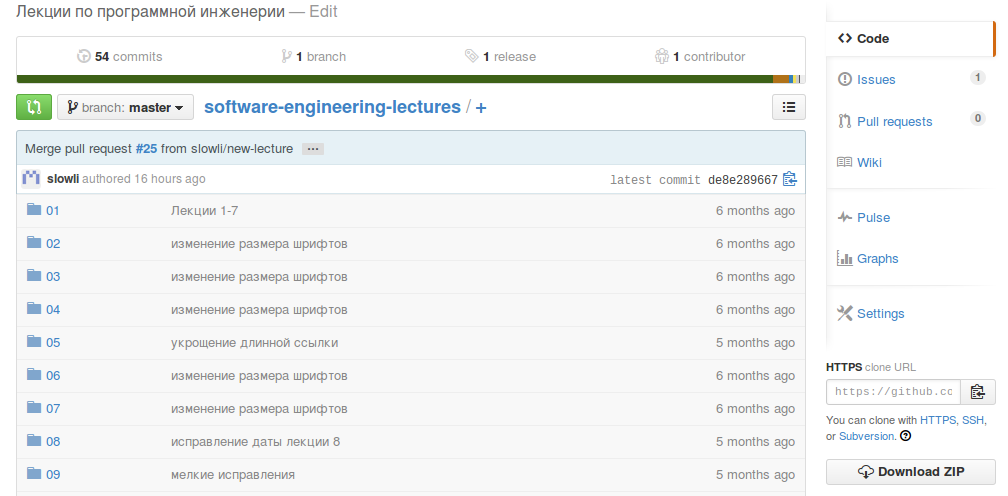
\includegraphics[scale=1.0]{fig-github.png}};

	\node<2> at (-4em,-2.75em) [border,minimum width=35em,minimum height=16em] {%
		\Large{Список файлов} \\ (для просомотра и редактирования)};

	\node<3>(commits) at (-16.75em,8.4em) [border,minimum width=6.5em,minimum height=1.5em] {};
	\node<3> [label,below=0pt of commits] {операции фиксации \\ в текущей ветви};

	\node<4>(branch) at (-16.5em,6.15em) [border,minimum width=6.5em,minimum height=1.5em] {};
	\node<4> [label,below=0pt of branch] {выбор ветви};

	\node<5>(release) at (0em,8.4em) [border,minimum width=6.5em,minimum height=1.5em] {};
	\node<5> [label,below=0pt of release] {создание и \\ скачивание выпусков};

	\node<6>(issue) at (17.8em,7.35em) [border,minimum width=7.5em,minimum height=1.5em] {};
	\node<6> [label,below=0pt of issue] {работа с запросами \\ на изменение};

	\node<7>(url) at (17.8em,-5.75em) [border,minimum width=8.5em,minimum height=2.5em] {};
	\node<7> [label,above=0pt of url,anchor=south east] {ссылка для \\ клонирования};

	\node<8>(download) at (17.8em,-9.75em) [border,minimum width=8.5em,minimum height=1.5em] {};
	\node<8> [label,above=0pt of download,anchor=south east] {скачивание основной \\ версии репозитория};
\end{tikz*}

		\else
			{\small\begin{tikz*}[%
	every node/.style={align=center},
	border/.style={rectangle,thick,draw=red,font=\color{red}},
	label/.style={font=\color{red}\small,fill=white}
]
	\node(a) {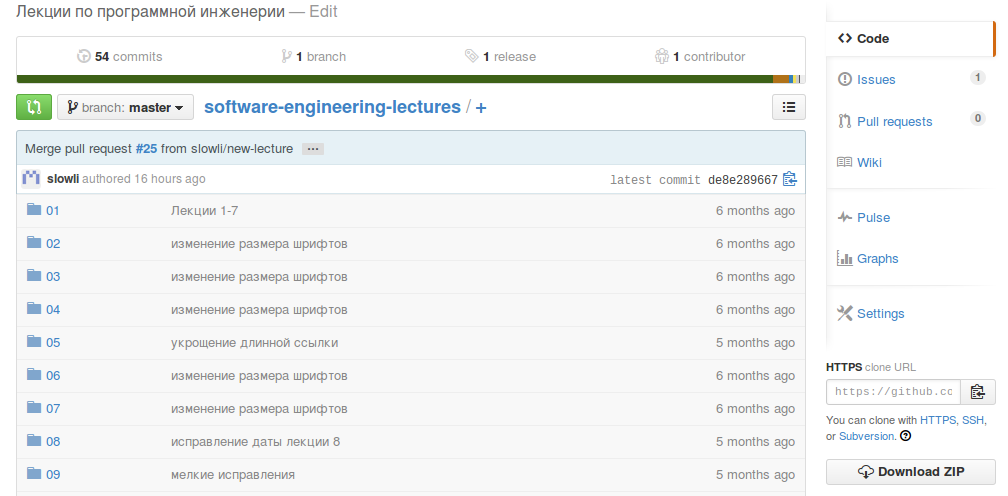
\includegraphics[scale=0.4]{fig-github.png}};

	\node<2> at (-4em,-2.75em) [border,minimum width=35em,minimum height=16em] {%
		\Large{Список файлов} \\ (для просомотра и редактирования)};

	\node<3>(commits) at (-16.5em,8.25em) [border,minimum width=6.5em,minimum height=1.5em] {};
	\node<3> [label,below=0pt of commits] {операции фиксации \\ в текущей ветви};

	\node<4>(branch) at (-16.25em,6em) [border,minimum width=6.5em,minimum height=1.5em] {};
	\node<4> [label,below=0pt of branch] {выбор ветви};

	\node<5>(release) at (0em,8.25em) [border,minimum width=6.5em,minimum height=1.5em] {};
	\node<5> [label,below=0pt of release] {создание и \\ скачивание выпусков};

	\node<6>(issue) at (17.5em,7.35em) [border,minimum width=7.5em,minimum height=1.5em] {};
	\node<6> [label,below=0pt of issue,anchor=north east] {работа с запросами \\ на изменение};

	\node<7>(url) at (17.5em,-5.75em) [border,minimum width=8.5em,minimum height=2.5em] {};
	\node<7> [label,above=0pt of url,anchor=south east] {ссылка для \\ клонирования};

	\node<8>(download) at (17.5em,-9.65em) [border,minimum width=8.5em,minimum height=1.5em] {};
	\node<8> [label,above=0pt of download,anchor=south east] {скачивание основной \\ версии репозитория};
\end{tikz*}
}
		\fi
	}

	\section{Заключение}

	\subsection{Выводы}
	
	\frame{
		\frametitle{Выводы}

		\begin{enumerate}
			\item
			Управление изменениями и версиями — важная часть управления разработкой~ПО, 
			в~особенности при~коллективной разработке.

			\item
			Движущей силой при модификации~ПО являются запросы на~изменение (change requests). 
			Инструменты для управления запросами могут быть самостоятельными приложениями 
			либо~встраиваться в~более общую систему управления разработкой.

			\item
			Системы управления версиями облегчают разработку~ПО в~нескольких направлениях 
			за~счет механизма ветвления / слияния. 

			\item
			Одна из наиболее популярных систем управления версиями — Git; 
			для~нее существуют веб-хостинги репозиториев, такие~как~GitHub.
		\end{enumerate}
	}
	
	\subsection{Материалы}
	
	\frame{
		\frametitle{Материалы}
		
		\begin{thebibliography}{9}
			\bibitem[1]{1}
			Sommerville, Ian
			\newblock Software Engineering.
			\newblock {\footnotesize Pearson, 2011. — 790 p.}

			\bibitem[2]{2}
			Лавріщева К.\,М. 
			\newblock Програмна інженерія (підручник). 
			\newblock {\footnotesize К., 2008. — 319 с.}

			\bibitem[3]{3}
			Eclipse Wiki
			\newblock EGit User Guide.
			\newblock {\footnotesize\url{http://wiki.eclipse.org/EGit/User_Guide} \\
			(руководство по использованию плагина Git для Eclipse)}
		\end{thebibliography}
	}
	
	\frame{
		\frametitle{}
		
		\begin{center}
			\Huge Спасибо за внимание!
		\end{center}
	}

\end{document}

